\chapter{Vyhodnocení systému}
\label{vysledky}

Tato kapitola popisuje způsob vyhodnocení vytvořeného systému a jeho výsledky. Vyhodnocování přesnosti analyzátorů proběhlo experimentálně. Součástí této kapitoly jsou experimenty se systémem, kterými se snažím zjistit další informace, jako například schopnost systému analyzovat data z jiných domén. Pro tento systém je velice důležitý dostatek dat, proto je zde jejich množství sepsané a porovnané. Poslední část demonstruje použití vytvořeného systému.

Výsledky jsou porovnány s dalšími dostupnými publikacemi.


\section{Datová sada}


Celkově se podařilo nasbírat poměrně velké množství recenzí. Pro porovnání s dalšími publikacemi, tato česká práce \cite{cz_dataset} používá datovou sadu o velikosti 21 tisíc recenzí, anglická~\cite{en_dataset} používá 50 tisíc recenzí. Datová sada použita v anglické práci je tvořena recenzemi z~\emph{imdb.com}, tato datová sada je pro analýzu sentimentu využívána velice často, knihovna \emph{Pytorch} má vytvořenou třídu pro stažení a práci s touto datovou sadou. Mými zdroji dat byly weby \emph{čsfd.cz} a \emph{fdb.cz} pro české recenze. Zdroji anglických recenzí se staly weby \emph{imdb.com} a \emph{rottentomatoes.com}. Celkové počty nasbíraných recenzí z každého portálu jsou sepsány v~tabulce~\ref{tab:table1.1}. 

Data byla po jejich získání ukládána do databáze (tabulka \emph{reviews}). Pro trénování analyzátorů byla data uložena do lokálního souboru ve formátu JSON. Z databáze byly použity pouze záznamy, které měly neprázdný text recenze a obsahovaly číselné hodnocení autora.

Recenze byly ze všech webových portálů stahovány s číselným hodnocením autora recenze. Tyto hodnocení byly nejprve normalizovány na desetinné číslo od nuly po jedničku. Recenze byly dále rozděleny podle tohoto hodnocení na pozitivní a negativní. Negativní recenze byly všechny ty, které měly hodnocení menší nebo rovno 0.5. Pozitivní byly ty, které měly hodnocení větší než 0.5. Tímto byla vytvořena datová sada pro analyzátor polarity (pozitivní / negativní). 

Stejná data byla využita i pro vytvoření datové sady pro klasifikátor míry pozitivity (jedna až pět hvězdiček). Jednotlivé recenze byly rozděleny do pěti kategorií podle uživatelského hodnocení s krokem 0.2. 

Recenze byly dále rozděleny na trénovací (60\%), validační (15\%) a testovací (25\%). Validační data jsou využita již při trénování ke zjištění přesnosti (\emph{accuracy}) a ztráty (\emph{loss}). Tyto hodnoty jsou využity k vybrání epochy ve které byl model nejúspěšnější, tento model je uložen. Testovací data jsou použita až na konci trénování k detailnějšímu přehledu o~úspěšnosti modelu.

Všechny recenze jsou uloženy v původním stavu, předzpracovány jsou až v průběhu trénování / analýzy.




\FloatBarrier
\begin{table}[h!]
  \begin{center}
    \caption{Počet recenzí pro polaritní analyzátor a analyzátor míry polarity}
    \label{tab:table1.1}
    \begin{tabular}{l|r|r|r}
      \textbf{Zdroj} & \textbf{Pozitivní} & \textbf{Negativní} & \textbf{Celkem}\\ 
      \hline
      \textbf{IMDb} & 1\,811\,198 & 855\,672 & 2\,666\,870\\ 
      \textbf{Rotten Tomatoes} & 5\,098 & 74\,270 & 79\,368 \\ 
      \textbf{ČSFD} & 239\,290 & 758\,021 & 997\,311\\ 
      \textbf{FDb} & 37\,055 & 108\,562 & 145\,617\\ 
      \textbf{Celkem} & 2\,092\,641 & 1\,796\,525 & 3\,889\,166\\ 
    \end{tabular}
  \end{center}
\end{table}
\FloatBarrier
\FloatBarrier

Data pro aspektové analyzátory byly anotovány ručně, proto jich je také mnohem méně, konkrétní počty v tabulkách \ref{tab:table1.2} pro češtinu a \ref{tab:table1.3} pro angličtinu. Opět pro srovnání, tato práce \cite{en_dataset2} má pro angličtinu čtyři datové sady, každá okolo 2\,000 vět.

Datová sada byla vytvořena následovně, nejprve byly vybrány náhodné recenze, poté byly rozděleny na věty pomocí nástrojů \emph{spacy} a \emph{nltk}. Jednotlivé věty byly ručně označeny pomocí nástroje \emph{brat}, který běží v prohlížeči. Server pro tento nástroj byl spouštěn lokálně na mém počítači. Každá věta byla anotována žádným až pěti aspekty a polaritou daného aspektu. Takto anotovaná data byla použita pro trénování analyzátorů polarity aspektů. Pro vytvoření datové sady k trénování analyzátorů detekujících aspekty ještě byly doplněny náhodné věty, datová sada pro analyzátory detekující aspekt byla tedy oproti hodnotám v~tabulkách dvakrát větší. 

\begin{table}[h!]
  \begin{center}
    \caption{Počet vět pro klasifikátory polarity aspektů v češtině}
    \label{tab:table1.2}
    \begin{tabular}{l|r|r|r}
      \textbf{Aspekt} & \textbf{Pozitivní} & \textbf{Negativní} & \textbf{Celkem}\\ 
      \hline
      \textbf{Herec} & 127 & 107 & 234\\ 
      \textbf{Postava} & 69 & 69 & 138 \\ 
      \textbf{Audio vizuální efekty} & 97 & 78 & 175\\ 
      \textbf{Příběh} & 81 & 81 & 162\\ 
      \textbf{Zkušenost} & 79 & 83 & 162\\ 
      \textbf{Celkem} & 453 & 418 & 871\\ 
    \end{tabular}
  \end{center}
\end{table}
\FloatBarrier
\begin{table}[h!]
  \begin{center}
    \caption{Počet vět pro klasifikátory polarity aspektů v angličtině}
    \label{tab:table1.3}
    \begin{tabular}{l|r|r|r}
      \textbf{Aspekt} & \textbf{Pozitivní} & \textbf{Negativní} & \textbf{Celkem}\\ 
      \hline
      \textbf{Herec} & 125 & 127 & 252\\ 
      \textbf{Postava} & 89 & 92 & 181 \\ 
      \textbf{Audio vizuální efekty} & 107 & 99 & 206\\ 
      \textbf{Příběh} & 164 & 168 & 332\\ 
      \textbf{Zkušenost} & 104 & 107 & 211\\ 
      \textbf{Celkem} & 589 & 593 & 1\,182\\ 
    \end{tabular}
  \end{center}
\end{table}
\FloatBarrier


\section{Maximální dosažená přesnost}
V této sekci jsou porovnány maximální dosažené přesnosti všech prováděných analýz vzhledem k použité metodě. Analyzátory byly trénovány na dříve popsaných datových sadách. Pro trénování analyzátorů založených na neuronové síti se data vybalancovala a rozdělila na trénovací, testovací a validační sady. Využita byla tedy většina dat. Oproti tomu při trénování analyzátorů založených na metodě podpůrných vektorů a naivní Bayesovské metodě, jsem byl z důvodu paměťové náročnosti způsobu trénování nucen vždy použít jen část trénovacích dat. 

Sledována je pouze přesnost (\emph{accuracy}) analyzátorů, která je definována jako poměr mezi počtem správných předpovědí (\emph{true positive}$+$\emph{true negative}) a celkovým počtem testovacích příkladů. Recenze byly před trénováním i testováním předzpracovány stejně jako bylo popsáno v kapitole \ref{implementace}. 

Snažím se zde odpovědět na otázku, zda-li je vůbec při analýze recenzí nutné používat relativně komplikovanější a náročnější metody jako jsou neuronové sítě, nebo stačí jednodušší metody jako podpůrné vektory nebo naivní Bayesova.




\subsection{Analýza polarity}

Prvním testovaným analyzátorem je analyzátor polarity. Analyzuje na úrovni celého dokumentu (recenze) a přiřazuje mu pozitivní nebo negativní třídu.
\FloatBarrier
\begin{table}[h!]
  \begin{center}
    \caption{Maximální přesnost použitých metod}
    \label{tab:table1.4}
    \begin{tabular}{l|l|l}
      \textbf{Metoda} &  \multicolumn{2}{l}{\textbf{Přesnost (\emph{Accuracy})}}\\ 
      \hline
      \textbf & CZ & EN \\ 
      \textbf{Neuronová síť (oboustranné LSTM)} & 0.81 & 0.88  \\ 
      \textbf{Metoda podpůrných vektorů} & 0.80 & 0.83 \\ 
      \textbf{Naivní Bayesovská metoda} & 0.69 & 0.69 \\ 
     \end{tabular}
  \end{center}
\end{table}
Z tabulky \ref{tab:table1.4} je patrné, že nejvyšší přesnost má dle očekávání systém založený na hlubokém učení. Z tohoto důvodu byl zvolen pro automatizovanou analýzu recenzí. Tento klasifikátor (obzvlášť pro angličtinu) dosáhl poměrně vysoké přesnosti, za nejmodernějšími systémy však ještě zaostává. Nejlepších výsledků by se pravděpodobně dosáhlo využitím systému jako je BERT a jeho doladěním na doménu filmových recenzí. Chtěl jsem si však klasifikátor z osobních důvodů implementovat sám, proto jsem se vydal touhle cestou.

Porovnáním přesností lze vidět, že metoda podpůrných vektorů moc nezaostává a její přesnost by byla přijatelná. V tomto případě by tedy asi nebyla potřeba využívat komplikovanějších metod.  
\FloatBarrier


\subsection{Analýza míry pozitivity}
Druhým typem analyzátoru je analyzátor míry pozitivity. Také analyzuje na úrovní dokumentu, přiřazuje jednu z pěti tříd (jedna až pět hvězd).
\FloatBarrier
\begin{table}[h!]
  \begin{center}
    \caption{Maximální přesnost použitých metod}
    \label{tab:table1.5}
    \begin{tabular}{l|l|l}
      \textbf{Metoda} &  \multicolumn{2}{l}{\textbf{Přesnost (\emph{Accuracy})}}\\ 
      \hline
      \textbf & CZ & EN \\ 
      \textbf{Neuronová síť (oboustranné LSTM)} & 0.62 & 0.55  \\ 
      \textbf{Metoda podpůrných vektorů} & 0.46 & 0.53 \\ 
      \textbf{Naivní Bayesovská metoda} & 0.45 & 0.52 \\ 
     \end{tabular}
  \end{center}
\end{table}
\FloatBarrier
Pro automatizovanou analýzu je opět používán analyzátor založený na hlubokém učení kvůli jeho přesnosti. Ostatní metody však moc nezaostávají, takže by byly použitelné také. Hned na první pohled lze v tabulce \ref{tab:table1.5} vidět, že oproti analýze polarity mají všechny metody přesnost nižší. To se dá očekávat, protože tento typ klasifikace je obtížnější. 
Z~důvodu poměrně velké změny v přesnosti jsem se však rozhodl analyzovat chyby hlouběji. Analýza chyb byla provedena na anglické datové sadě s využitím klasifikátoru založeném na hlubokém učení.
Celkový počet testovacích příkladů byl 146\,664, z toho bylo 60\,565 chyb (to znamená přesnost 0.58). U každé chyby bylo zaznamenáno, jestli se klasifikátor dopustil chyby pouze o jednu hvězdu nebo více. Výsledky jsou následující (nalevo od pomlčky je předpokládaná odpověď analyzátoru).

\textbf{Počet chyb o jednu hvězdu:}
\begin{itemize}
    \item jedna hvězda - 792
    \item dvě hvězdy - 4\,132
    \item tři hvězdy - 10\,404
    \item čtyři hvězdy - 4\,921
    \item pět hvězd - 9\,361
\end{itemize}

\textbf{Počet chyb o více než jednu hvězdu:}
\begin{itemize}
    \item jedna hvězda - 4\,434
    \item dvě hvězdy - 9\,890
    \item tři hvězdy - 6\,324
    \item čtyři hvězdy - 7\,960
    \item pět hvězd - 2\,347
\end{itemize}

Celkově bylo 29\,610 chyb o jednu hvězdu, to je 48\,\% všech chyb. Předpokládám, že tohle je z důvodu malého rozdílu v obsahu textu recenzí mezi těmi blízko u sebe v hodnocení.

\FloatBarrier

\subsection{Analýza aspektů}
Aspektová analýza se skládá ze dvou úkolů, detekci aspektu (výsledky v tabulce \ref{tab:table1.6}) a~určení polarity daného aspektu (tabulka \ref{tab:table1.7}).
\FloatBarrier
\begin{table}[h!]
  \begin{center}
    \caption{Detekce aspektu}
    \label{tab:table1.6}
    \begin{tabular}{l|l|l}
      \textbf{Metoda} &  \multicolumn{2}{l}{\textbf{Přesnost (\emph{Accuracy})}}\\ 
      \hline
      \textbf & CZ & EN \\ 
      \textbf{Neuronová síť (oboustranné LSTM)} & 0.72 & 0.71  \\ 
      \textbf{Metoda podpůrných vektorů} & 0.74 & 0.73 \\ 
      \textbf{Naivní Bayesovská metoda} & 0.72 & 0.66 \\ 
     \end{tabular}
  \end{center}
\end{table}
\FloatBarrier


\begin{table}[h!]
  \begin{center}
    \caption{Určení polarity aspektu}
    \label{tab:table1.7}
    \begin{tabular}{l|l|l}
      \textbf{Metoda} &  \multicolumn{2}{l}{\textbf{Přesnost (\emph{Accuracy})}}\\ % <-- added & and content for each column
      %$\alpha$ & $\beta$ & $\gamma$ & $\delta$ \\ % <--
      \hline
      \textbf & CZ & EN \\ 
      \textbf{Neuronová síť (oboustranné LSTM)} & 0.69 & 0.69  \\ 
      \textbf{Metoda podpůrných vektorů} & 0.65 & 0.68 \\ 
      \textbf{Naivní Bayesovská metoda} & 0.64 & 0.67 \\ 
     \end{tabular}
  \end{center}
\end{table}
\FloatBarrier

Na české datové sadě byla přesnost zjištěna pro aspekt \uv{herec}, na anglické pro aspekt \uv{příběh}. Tyto aspekty byly vybrány, protože mají nejvíce anotovaných vět. Důvodem je nutnost rozdělení datových sad na trénovací a testovací části. Klasifikátory ostatních aspektů mají velice podobnou přesnost.

Z výsledků je patrné, že všechny metody mají velice podobné výsledky. Tohle je způsobeno menším počtem dat. Pro automatickou analýzu je opět zvolena neuronová síť. 

\section{Využití analyzátorů v jiných doménách}
Těmito experimenty je testována schopnost polaritních analyzátorů pracovat na datech z~jiných domén. Filmových recenzí je obrovské množství, navíc jsou již anotovány autorem. Kdyby se tedy ukázalo, že analyzátory natrénované na těchto datech jsou úspěšné i v jiných doménách, mohlo by  to ulehčit práci s hledáním trénovacích dat.  Testy byly provedeny na následujících datových sadách (vyvážená byla pouze sada Mallcz):
\begin{itemize}
    \item Facebook - česká datová sada, necelých 5\,000 příspěvků.
    \item Mallcz - česká datová sada, použito 10\,000 recenzí.
    \item Hudební nástroje - anglická datová sada, jedná se o recenze z webového portálu \emph{Amazon}. Přes 10\,000 recenzí.
    \item Automobilový průmysl - anglická datová sada, jedná se o recenze z webového portálu \emph{Amazon}. Přes 20\,000 recenzí.
    \end{itemize}

\FloatBarrier
\begin{table}[h!]
  \begin{center}
    \caption{Polaritní analyzátory v jiných doménách}
    \label{tab:table1.8}
    \begin{tabular}{l|l|l|l|l}
      \textbf{Metoda} &  \multicolumn{4}{l}{\textbf{Přesnost (\emph{Accuracy})}}\\ % <-- added & and content for each column
      %$\alpha$ & $\beta$ & $\gamma$ & $\delta$ \\ % <--
      \hline
      \textbf & Facebook & Mallcz & Hudební nástroje & Automobilový průmysl \\ 
      \textbf{Neuronová síť} & 0.57 & 0.51 & 0.83 & 0.75  \\ 
      \textbf{Podpůr. vekt.} & 0.52 & 0.47 & 0.77 & 0.59 \\  \textbf{Naivní Bayes.} & 0.43 & 0.45 & 0.14 & 0.12 \\ 
     \end{tabular}
  \end{center}
\end{table}
\FloatBarrier
Ve výsledcích jde vidět (tabulka \ref{tab:table1.8}), že obecně jsou úspěšnější anglické datové sady. To bude pravděpodobně tím, že čeština je bohatější jazyk a tím těžší pro klasifikátor na naučení. 

Přesnost naivní bayesovské metody v anglických datových sadách je opravdu zvláštní. Všechno bylo zkontrolováno, test byl proveden několikrát a vždy vyšel stejně. 

Z výsledků vyplývá, že analyzátory kromě třech případů nejsou velice úspěšné. Filmové recenze jsou nejspíše příliš konkrétní doménou a pro trénování analyzátorů do jiných domén se moc nehodí. Klasifikátory by se daly doladit (dotrénovat na konkrétní doméně) a tím zvýšit jejich přesnost. Toto už však testováno nebylo.  

\FloatBarrier

\section{Přesnost v závislosti na velikosti trénovacích dat}
Zde chci porovnat přesnosti metod polaritní analýzy v závislosti na počtu trénovacích příkladů. Cílem je zjistit potřebné množství dat pro natrénovaní analýzátoru s přijatelnou přesností. Využity jsou části již popsaných datových sad. Testování probíhalo na náhodně vybrané sadě o velikosti 100\,000 recenzí. Trénovací sada (také vytvořená náhodně) se postupně zvětšovala. 

\FloatBarrier
\begin{table}[h!]
  \begin{center}
    \caption{Přesnost v závislosti na velikosti trénovacích dat}
    \label{tab:table1.9}
    \begin{tabular}{r|r|r|r|r|r|r}
      \textbf{Počet recenzí} &  \multicolumn{2}{l}{\textbf{Neuronová síť}} & \multicolumn{2}{l}{\textbf{SVM}} & \multicolumn{2}{l}{\textbf{Bayes}}\\ 
      \hline
      \textbf & CZ & EN & CZ & EN & CZ & EN \\ 
      \textbf{50} & 0.65 & 0.54 & 0.66 & 0.69 & 0.54 & 0.52  \\ 
      \textbf{100} & 0.66 & 0.46 & 0.67 & 0.71 & 0.62 & 0.66 \\  
      \textbf{200} & 0.70 & 0.62 & 0.77 & 0.70 & 0.71 & 0.64 \\ 
      \textbf{500} & 0.70 & 0.67 & 0.78 & 0.76 & 0.72 & 0.67 \\ 
      \textbf{1000} & 0.72 & 0.65 & 0.77 & 0.77 & 0.74 & 0.68 \\ 
      \textbf{2000} & 0.72 & 0.66 & 0.80 & 0.78 & 0.72 & 0.68 \\ 
      \textbf{5000} & 0.74 & 0.68 & 0.79 & 0.80 & 0.73 & 0.69 \\ 
      \textbf{10000} & 0.78 & 0.75 & 0.81 & 0.80 & 0.75 & 0.71 \\ 
     \end{tabular}
  \end{center}
\end{table}
\FloatBarrier

V tabulce \ref{tab:table1.9} jde vidět, že po trénování na datové sadě o velikosti 5\,000 recenzí již za svým maximem zaostává pouze klasifikátor založený na neuronové síti. Z toho vyplývá, že pro menší datové sady je lepší využít jiné metody. 

Cekově z výsledků vyplývá, že pro natrénování poměrně přijatelně přesného klasifikátoru není potřeba příliš mnoho dat (v poměru k počtu dostupných recenzí). 

\section{Demonstrace systému}
V této sekci chci ukázat několik příkladů jak se dá vytvořený systém využít a jaké informace se dají za jeho pomoci získat. 


\subsection{Správné vydání filmu}

Pro analýzu dat byl použit dříve popsaný graf polarity (kapitola \ref{moviedetail}). 
\begin{figure}[!htb]
\label{ad_astra}
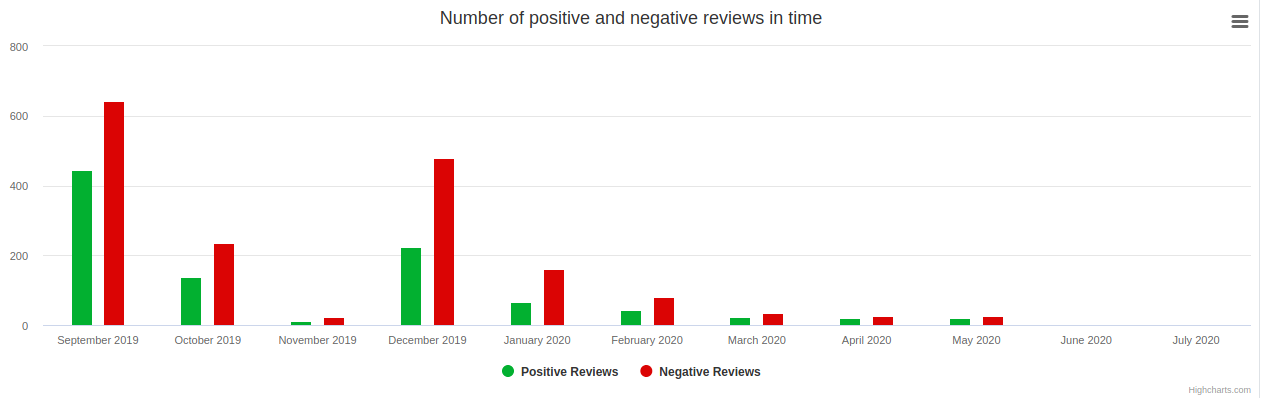
\includegraphics[width=\textwidth]{ad_astra.png}
\caption{Počet pozitivních a negativních hodnocení v čase pro film \emph{Ad Astra}}
\end{figure}

\begin{figure}[!htb]
\label{cats}
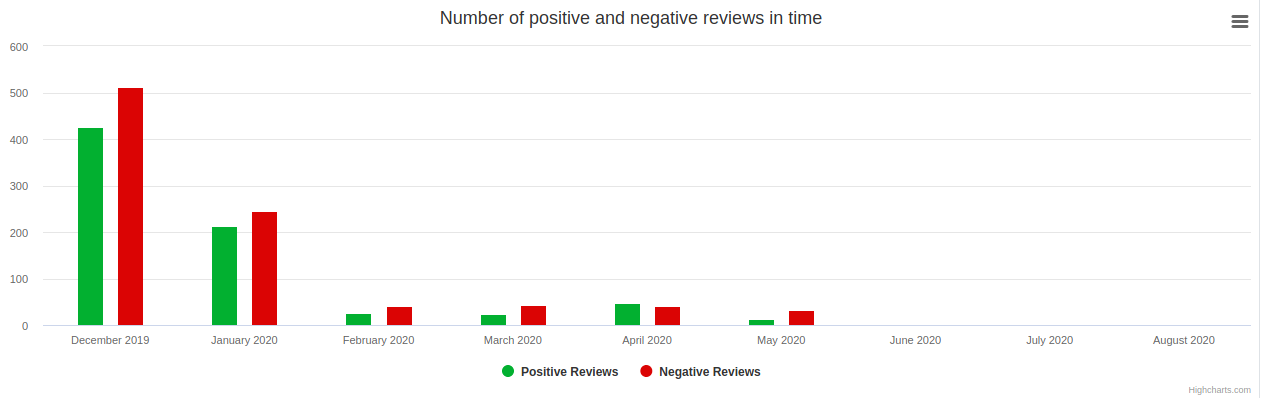
\includegraphics[width=\textwidth]{cats.png}
\caption{Počet pozitivních a negativních hodnocení v čase pro film \emph{Cats}}
\end{figure}

Oba filmy jsou poměrně neúspěšné, celkové hodnocení mají okolo 50\,\%. Pohledem na oba grafy \ref{ad_astra} a \ref{cats} lze zjisti, že jejich průběhy jsou velice podobné. Po vydání poměrně vysoká popularita (velký počet pozitivních i negativních recenzí). Po čase však tato popularita rapidně klesá. Pohledem na graf \ref{ad_astra} lze vidět v prosinci 2019 velký nárůst popularity. Po krátkém zkoumání lze zjistit, že v tomto měsíci byl film vydán na DVD, to je zhruba 3~měsíce po vydání. Tento fakt velice pozvedl popularitu. Oproti tomu film \emph{Cats} (graf \ref{cats}) žádný takový nárůst nemá. DVD tohoto filmu bylo totiž vydáno až téměř po půl roce od vydání, podle grafů tohle byla chyba. Po tak dlouho době již vyprší nadšení z nového filmu a jeho marketingové kampaně.  



\subsection{Pravdivost celkových hodnocení}
U převážné většiny titulů je originální celkové hodnocení a celkové hodnocení vytvořené systémem velice podobné. Zde prezentuji jeden příklad kdy tohle není pravdou. 

\begin{figure}[!htb]
\label{starwars}
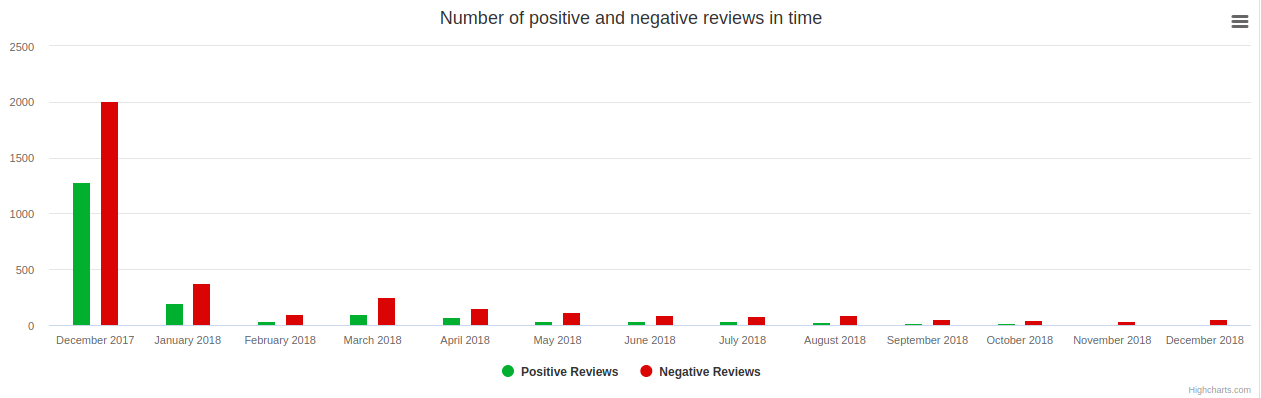
\includegraphics[width=\textwidth]{last_jedi.png}
\caption{Počet pozitivních a negativních hodnocení v čase pro film \emph{Star Wars: Episode VIII - The Last Jedi (2017)}}
\end{figure}

Již na první pohled lze v grafu \ref{starwars} vidět, že se nejedná o velice úspěšný film. Celkové hodnocení systému(vytvořené průměrem hodnocení uživatelů \emph{imdb}) je 41\,\%. Při návštěvě webových stránek \emph{imdb} však vidíme hodnocení 7/10. Velice podobný případ lze nalézt i~u~2~roky staršího předchůdce \emph{Star Wars: Episode VII - The Force Awakens}. Tam systém tvrdí 57\,\%, na \emph{imdb} je však napsáno 7,9/10.



\chapter{Závěr}
\label{zaver}

Cílem této práce bylo navrhnout a implementovat systém schopný pravidelně získávat, indexovat a analyzovat recenze filmů v češtině a angličtině. Cíl práce byl splněn. 

V práci je prostudována teorie základních i pokročilých metod pro rozpoznávání postojů a zpracování přirozeného jazyka. Dále byly určeny vhodné zdroje recenzí filmů a seriálů pro oba jazyky. Těmito zdroji se staly webové portály \emph{csfd.cz}, \emph{fdb.cz}, \emph{imdb.com} a \emph{rottentomatoes.com}. Recenze z těchto portálů jsou pravidelně stahovány a indexovány v relační databázi. Současně jsou v databázi téměř čtyři miliony recenzí filmů a seriálů. 

Využitím těchto recenzí byly natrénovány analyzátory třech typů. Prvním z nich je analyzátor polarity na úrovni dokumentu určující celkový postoj recenze (pozitivní / negativní). Tento analyzátor dosahuje přesnosti až 88\,\% pro angličtinu a 81\,\% pro češtinu. Druhým typem je analyzátor míry pozitivity pracující také na úrovni dokumentu, tento analyzátor rozděluje recenze do pěti tříd (jedna až pět hvězd). Tato analýza dává detailnější informace o recenzi, ale má nižší přesnost, a to 55\,\% pro angličtinu a 62\,\% pro češtinu. Po detailnější analýze chyb toho klasifikátoru se ukázalo, že má problém s rozlišením recenzí s podobným hodnocením (například recenze s pěti a čtyřmi hvězdičkami). Posledním typem je analýza aspektů, která dává nejdetailnější informace. Předem bylo definováno pět aspektů, které jsou u recenzí sledovány (herec, postava, příběh, audio vizuální efekty a zkušenost diváka). Analýza je rozdělena do dvou kroků, nejprve jsou jednotlivé aspekty nalezeny a poté ohodnoceny polaritou (pozitivní / negativní).

Výsledky z automaticky prováděných analýz jsou ukládány do relační databáze a zobrazovány ve webovém rozhraní (\url{http://athena1.fit.vutbr.cz:8078/}). Rozhraní uživateli nabízí vyhledávat a filtrovat filmy a seriály. Každý film má vytvořenou časovou osu názorů na daný film s detailní analýzou jednotlivých recenzí týkajících se filmu. Dále jsou sledovány trendy titulů podle žánru, země původu a jestli je daný titul film či seriál. 

V práci bych pokračoval anotací dalších dat pro aspektovou analýzu, tím by se zvýšila její přesnost, popřípadě bych otestoval další metody implementace analyzátorů. Dále bych rád udělal hezčí a dynamičtější webové rozhraní. Pro přilákání uživatelů na platformu by bylo dobré jim dát možnost přímo interagovat s klasifikátory, dnes je téma strojového učení velice populární.    